\section{Design and Implementation}
\label{sec.design}

\begin{figure*}
\centering
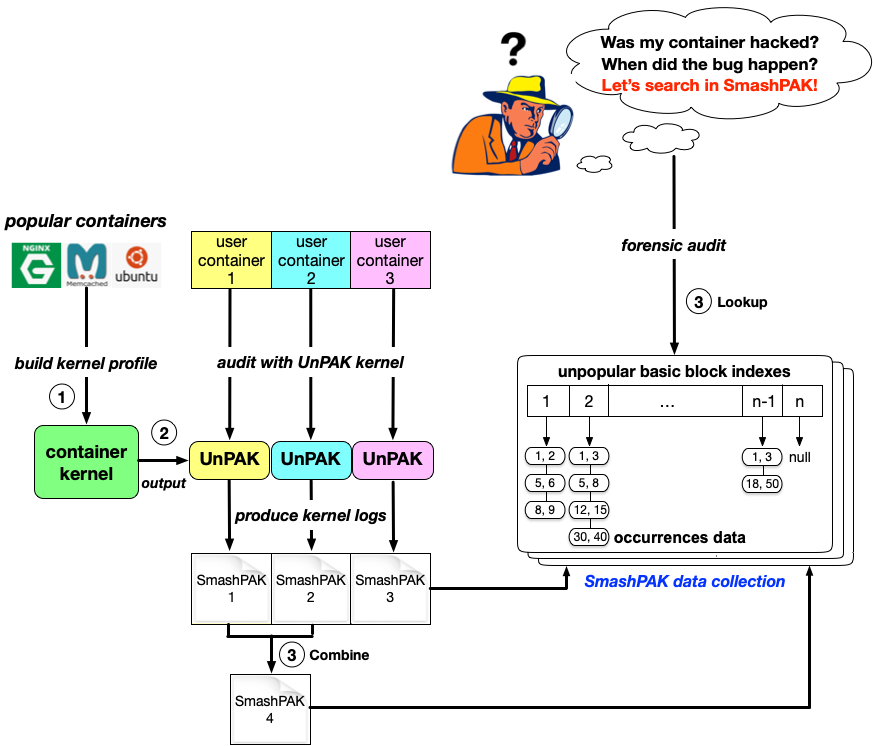
\includegraphics[width=2.2\columnwidth]{diagram/SmashPAK.png}
\caption{\small Audit Containers with SmashPAK}
\label{fig:design}
\end{figure*}

As described in Section 2, the container kernel security auditing method we propose requires execution of three main steps, as illustrated in Figure \ref{fig:design}. 
In Step 1, we developed a systematic method to collect data on the most frequently used container paths (referred to here as popularity data) and built a kernel profile. 
In Step 2, we used the profile to identify the unpopular paths in the kernel that contain more bugs, and to automatically modify the kernel to produce UnPAK. 
UnPAK marks each attempt to access unpopular paths, thus generating a log of likely locations for exploits. 
Most importantly, in Step 3, we introduced a novel data structure, called \textbf{SmashPAK} to store, update, and query the kernel logs to perform efficient forensic auditing for containers. 
The box in the bottom right of the diagram shows how SmashPAK data is characterized and indexed into a database that allows for easy access and searching.

\noindent
\textit{\textbf{Step 1: Build the kernel profile}}

This step builds a kernel trace profile by identifying the lines of code executed  in the  container kernel while running the default / regular workload defined in the “CMD” section of the configuration files (Dockerfiles) that come with the container images. It builds the popular paths kernel profile by running a set of containers ranked as “most popular” based on the number of user downloads from DockerHub [4]. The profile provides data on both the popular and unpopular code in the container kernel, which is required to identify the right place to do kernel auditing. 

We chose LinuxKit \cite{LinuxKit} VM as the base environment to build this profiles, because it provides an isolated space that helps eliminate noises as much as possible. 
LinuxKit  can run container images with minimal functionality, reducing most of the background noises experienced in a Native Linux host OS. 
In addition, LinuxKit was designed to run Docker containers, and supports customized container kernels, which allows us to use a Gcov \cite{gcov} enabled Linux kernel to profile the kernel trace.

Here is how Step 1 works:
\begin{enumerate}
	\item The Linux kernel used to run the Docker containers is recompiled with the Gcov \cite{gcov} kernel profiling feature enabled. 
	\item Our tool automatically generates the configuration file for the Gcov-enabled LinuxKit. 
	\item The LinuxKit virtual machine is booted and a script automatically starts running the workload of the task container. Our code collects the kernel trace data, and, by the end of the run, transfers the data to the host system. 
	\item We then use the lcov \cite{lcov} tool to process the kernel trace data collected from the host system. 
\end{enumerate}

\noindent
\textit{\textbf{Step 2: Produce the UnPAK auditing kernel}}

We use the kernel profile built by Step 1 to find and mark the rarely used unpopular paths, and to modify the container kernel to generate forensic logs when it reaches these paths. The resulting tailored kernel is called UnPAK. As it was essential to collect this logging data on running containers, we needed to ensure that UnPAK could  run default workloads without requiring any changes to the containers themselves. 

Step 2 was implemented as follows: 
\begin{enumerate}
	\item The Clang C compiler from the Clang / LLVM project \cite{llvm}, along with a BEAR \cite{bear} tool compiles the Linux kernel source. Using BEAR, we can generate a compilation database containing all the compile flags and options needed. 
	\item The Clang analyzer performs static analysis on the kernel source code to obtain the control flow graph for each function in the files. The analyzer leverages Clang’s LibTooling \cite{clang-libtooling} to construct the AST tree from the kernel source code, and then obtain the control flow graph. With this graph, we can identify the corresponding source line number for each basic block. Furthermore, the beginning lines of all the blocks in the source files are candidates for places to add security logging code. Here, a \textbf{\textit{basic block}} refers to a straight-line code sequence with no branches in except at the entry and no branches out except at the exit. Thus, if a basic block is unpopular, it is sufficient to insert only one piece of secure logging code where it begins to alert users of any attempt to reach that code. This approach can optimize instrumentation by  avoiding redundancy in code injection. 
	\item Our kernel modifications are based on both the basic blocks, and the collected popular paths data. If none of the lines in a basic block are in the popular paths data, the block is considered unpopular, and the  instrumenting tool will add the security logging code, a kvm hypercall from the LinuxKit kernel into the host Linux kernel at the beginning. If we discover that an entire function has no lines in the popular paths data, we consider this an unpopular function, and just add our security logging code once where it starts.  
\end{enumerate}

%\begin{table}
%\caption{Instrumentation code added to UnPAK}
%\label{tab:kernel_instrumentation}
%\begin{tabular}{c|c|c|c}
% kernel dir & unpopular & popular & total lines \\
% & functions & functions & inserted \\
% \hline
% arch & 1502 & 931 & 3325 \\
% \hline
% block & 774 & 245 & 1035 \\
% \hline
% crypto & 527 & 121 & 656 \\ 
% \hline
% drivers & 6290 & 2584 & 13305 \\
% \hline
% fs & 2108 & 1404 & 4883 \\
% \hline
% ipc & 198 & 42 & 249 \\
% \hline
% kernel & 3721 & 2120 & 6335 \\
% \hline
% mm & 1037 & 792 & 2954 \\
% \hline
% net & 4107 & 1746 & 7510 \\
% \hline
% security & 200 & 180 & 551 \\
% \hline
% \textbf{total} & \textbf{20464} & \textbf{10165} & \textbf{40803} \\
%\end{tabular}
%\end{table}
 
\noindent
\textit{\textbf{Step 3: Implement SmashPAK to enable forensic security auditing}}

\textit{\textbf{SmashPAK}} is a novel data structure designed to manage and process the kernel logs to enable users to inquire about when and where a bug occurred in the container kernel. 

A SmashPAK data structure is effectively implemented as an index of positions. In our case, these positions were unpopular basic blocks, 
each of which indexes into an occurrences data structure and is implemented as a series of range items.  Each range item contains a start time and end time. 
The special case of a start time = end time is permitted since it is common. Each occurrences data structure has a maximum fixed size.  
If a new range item is added to the structure, then the two existing range items with the smallest gap between them are combined.  

SmashPAK supports the following operations:
\begin{itemize}
	\item CreateSmashPAK(numindices, max\_occurrence\_size) -> returns an index with a NIL occurrence data structure in each position
	\item Lookup(index) -> returns the occurrence list for that index
	\item Add(index, occurrence\_list) -> adds a range\_item or occurrence\_list as described above.
	\item Combine(SmashPAKA, SmashPAKB) -> take each occurrence list at index i of both data structures and call Add.  The resulting SmashPAK combines information from each list.
\end{itemize}

A SmashPAK is a data structure that stores information about a sequence of items.  It is designed for quick lookups for parties that want to both store and update data efficiently.  
It is a lossy data structure, in that it does not provide perfect information.  For example, a SmashPAK may return information showing that accesses occurred between time X and Y, 
but not precisely how many accesses, or exactly when it occurred.  (This is somewhat similar to the limitations of gcov and similar tools, only extrapolated over a large scale.) 
Note that while there is some data loss with a SmashPAK, it does help to answer the most pressing question, ``Was this ever potentially exploited and if so, roughly when?''  
It does so with little to no cost of overhead.  An organization may choose to retain more granular SmashPAKs or the UnPAK information used to generate them for more finer-grained auditing capabilities.

The fact that SmashPAK data structures can also be combined offers a distinct advantage for container environments, where a large number of ephemeral containers are started and then later destroyed.  
The workload and the purpose of the container is the most critical part, so administrators will want to collect and combine data about instances to search them.  
To do so the SmashPAKs are co-located and the Combine function is called to combine them and produce a SmashPAK containing data from both. 
To show how combining works, take for example, the following scenario. If the maximum length is 4, and the items are [(1,2), (5,7), (10,19), (30,40)] and (44,50) is added, (5,7) and (10,19) are merged 
to give (5-19).  If (42,50) had been added instead, then it would have been merged into (30,40). 
Similarly, two occurrence lists may be merged by combining the lists and then iteratively removing the smallest gaps.    

Once the SmashPAK database is established, a system administrator can easily check for evidence of an exploit every time a new CVE comes out.  
A user can inspect the corresponding kernel patch and then search via SmashPAK for the occurrences data structures at those indices.  
If they contain any entries, it will indicate times when the basic blocks were triggered and hence the CVE could have been exploited. 
This alerts both the system administrators and its security teams to take proper measures against malicious containers or potential attackers. 